%\documentclass{amsart}

\documentclass{book}
%\documentclass{amsart, tikz}
\usepackage{amssymb,latexsym,color,amsthm}

%allows for comment blocks and verbatim sections
\usepackage{verbatim}

%preserves tabs in verbatim sections. Good for including source code in documents.
\usepackage{moreverb}

\usepackage{graphicx}

\definecolor{Dark}{gray}{.20}
\definecolor{Light}{gray}{.80}
\newcommand{\commandline}[1]{\begin{center} \colorbox{Dark}{\textcolor{white}{#1}} \end{center}}
\newcommand{\exampleout}[1]{\begin{center} \colorbox{Light}{\textcolor{black}{#1}} \end{center}}

\newtheorem{ex}{Exercise}[chapter]
\begin{document}


\title{An Introduction to the UNIX Command Line}
\author{Brandon Tarquinio}

\maketitle
\tableofcontents
\newpage
\chapter{The Basics}

\section{Introduction}
In this workshop we will run through the basics of using $bash$ or some other Unix-like command line environment. $bash$ is the most popular of the different $shells$ (it is then default on most Linux distros and OSX) but most things we discuss will be universal to all shells for Unix-like computers.\footnote{For example Linux, OSX, FreeBSD. Also Cygwin provides a Unix-like environment for Windows computers.} We will run through enough of the basics that the blinking cursor of a shell is no longer daunting to you. This will include how to manipulate files and directories, $redirection$ and $pipes$, and how to run your programs for your classes. 


\section{Running a Command}
The general form of any command, for the most part, is as follows:
\commandline{commandname -arg1 -arg2 ... --longerargs ... input1 input2 ...}
Note that $arg$ is a common shortening of argument and that $longerargs$ is preceeded by two dashes while arg1 and arg2 are preceeded by only one.


The ''\dots" above are used to denote that we can have any number of args of the first type followed by any number of args of the other type followed by any number of input. \footnote{In actuality every command has a finite number of arguments it understands and you normally use a small subset of those. There might also be a limit on the number of input.}
Lets look at an example:
\commandline{head -v --lines=20 myfile}
We will go over \textbf{head}, along with many other commands, later but for now we just want to understand the general form of commands. 

Also note that the double dashed longerargs arguments will only work on Linux and cannot be used on Mac OSX for example. Generally there is an equivalent short arg version. For example we can run the following on Linux or OSX:
\commandline{head -v -n 20 myfile}
Which is exactly the same as our previous example. 

\section{Directories and Moving Around}

\subsection{Directory trees and pwd}
We will start by learning some commands to move around the directory tree. It is called a directory tree because it can be visualized as follows:
\begin{figure}[ht!]
	\centering
	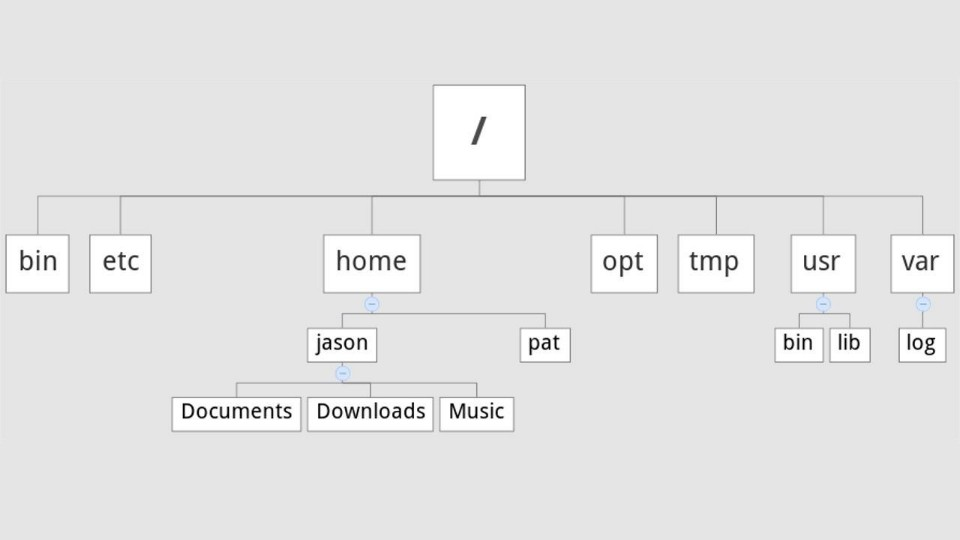
\includegraphics[width=90mm]{linux-directory-tree.jpg}
	\caption{An Example Linux Directory Tree.} 
\end{figure}

Each of the boxes in Figure 1 are directories and we call the directory ``$/$" $root$ since it is the root of our tree. In a command line enter:
	\commandline{pwd}
  This will \textbf{p}rint your current \textbf{w}orking \textbf{d}irectory. For example if we were in the directory $jason$ and typed \textbf{pwd} we would get the following:
	\exampleout {/home/jason}
  Note that your $prompt$ (the thing that is printed after every command which allows you to enter the next) might be set up to display this information. The prompt is something you can change to your liking to include, or not include, a bunch of information but this is beyond the scope of this workshop. \\

\subsection{Listing the contents of a Directory}
To \textbf{ls}it all the files in your current working directory enter:
	\commandline{ls}
In our example we get the following printed to the terminal:
	\exampleout {Documents Downloads Music}
	Most shell environments can be set up ( and yours might already be) so that directories are printed with a different colour than files and soft links. We will be discussing the difference between files, soft links, and directories shortly. We can also specify to \textbf{ls} what directory we want to list the contents of with the following generic form:
  	\commandline{ls dirname}
For example:
	\commandline{ls /home}
will display the following:
	\exampleout{jason pat}

\subsection{Special Directory entries and shortcuts}
First we will define what the $Home$ directory is
\begin{itemize}
	\item Home: Every user has a home directory. When you log onto a terminal you will start in your home directory. Think of this as the root of the tree which is all of your personal files.
	\item ``.": This represents the current directory and is an actually entry in every directory.
	\item ``..": This represents the parent of the current directory and is also an actually entry in the current directory.
\end{itemize}

\begin{ex} 
	Lets explore the concept of home by running the following commands:
	\commandline{pwd}
	\commandline{echo \$HOME}
	\commandline{echo \~{} }
	What did you find? Note that ``\~{}", the tilde symbol which is located to the left of the 1 on your keyboard, and ``\$HOME" are shortcuts to your home directory. Remember ``\~{}" since it will be used a lot.
\end{ex}
\begin{ex}
	I said before that ``." and ``.." are actual entries in every directory but when we ran \textbf{ls} earlier we did not see them. The -a argument\footnote{The a is short for all.} for \textbf{ls} will solve this mystery. Enter the following commands:
	\commandline{ls -a}
	\commandline{ls -a .}
	\commandline{ls -a \~{}}
	\commandline{ls -a \$HOME}
	\commandline{ls ..}
Does the output make sense? As a challenge question what will the following command do? (Try to think it out before running it!):
	\commandline{ls ././././}
\end{ex}

\subsection{Relative vs Absolute Path Names}
We need to learn one more important concept about UNIX files and directories before moving on to learning a bunch of commands and how we can use them to help us program. \\
Suppose we are in the directory /home in our directory tree figure and we wanted to list the contents of the jason directory. We can do this in two ways:
\commandline{ls jason}
or
\commandline{ls /home/jason}
In the later we used the \textbf{absolute path name} which is the name of the file or directory prefixed by the path from ``/" to it. When we use absolute path names it no longer matters what are current working directory is e.g. we could have run the second command from any directory. In contrast, the first command will only list the contents of /home/jason if are current working directory is /home. This is because jason is a $relative path name$ since we assume the path begins in our current working directory. relative path names allows the user to remember and type less but require careful consideration of what your working directory currently is. 

\subsection{Changing your Current Working Directory}
We have talked a lot about current directories changing but have yet to figure out how to do so. We can \textbf{c}hange the \textbf{d}irectory with \textbf{cd} which has the following form:
\commandline{cd dirToChangeTo}
For example we can run:
\commandline{cd /}
And then:
\commandline{pwd}
and we will see:
\exampleout{/}
To change back to our previous directory with this shortcut:
\commandline{cd -}
To change to our home directory regardless of where we are we can simply type:
\commandline{cd}
Thus the default to \textbf{cd} is to change to the users home directory. \\
\begin{ex}
	Use \textbf{cd}, \textbf{pwd}, \textbf{ls} to explore the directory tree a bit. Becoming familiar and quick with this is key to become efficient with the command line since \textbf{cd} and \textbf{ls} are easily the two most used commands.
\end{ex}

\subsection{Making a Directory}
Now that we understand the directory tree and how to move around it we are ready to learn how to add to it. The general form of the command to \textbf{m}a\textbf{k}e a \textbf{dir}ectory is:
\commandline{mkdir newdirname1 newdirname2 ...}
\begin{ex}
	Run the following sequence, before the second and third call to \textbf{ls} think about what you would expect to see:
\commandline{clear}
\commandline{ls}
\commandline{mkdir FirstDir SecondDir}
\commandline{ls}
\commandline{mkdir FirstDir/Foo FirstDir/Foo2}
\commandline{ls FirstDir}
\textbf{clear} is a useful command that clears the screen.
\end{ex}
\begin{ex}
	\begin{enumerate}
			\item make a directory called ``.ghost".
			\item run:
				\commandline{ls}
				What happened?
			\item Can you think of a command we have learned to be able to see ``.ghost"? A directory or file that begins with a ``." is said to be a hidden file or directory. They are mostly used for configuration files. Do you see any hidden files in your home directory?
	\end{enumerate}
\end{ex}

\subsection{Deleting a Directory}
The program to \textbf{r}e\textbf{m}ove a \textbf{dir}ectory, \textbf{rm}, has the following form:
\commandline{rmdir dirname1 dirname2 ...}
This command will only work if the directories you are trying to delete are \textbf{empty}. An empty directory is a directory which only has no other entries but ``." and ``..". Thus dirname1 is empty if we run:
\commandline{ls dirname1}
and nothing appears. Note that this is not like windows where there is a recycle bin for files and folders that are deleted; in Unix when you delete something it is gone! In turn you should be very careful when you delete directories and files ( we will learn how to delete files and non-empty directories later).
\begin{ex}
	\begin{enumerate}
		\item Start by making sure you are in the home directory using \textbf{pwd} and \textbf{echo \~{}}. Also make sure you still have FirstDir and SecondDir by using \textbf{ls}.
		\item Use \textbf{rmdir} to delete SecondDir.
		\item Use \textbf{ls} to make sure it is gone.
		\item Make three new directories SecondDir, ThirdDir, and ThirdDir/Foo.
		\item Delete the three directories you just made. Did you have any issues? Can you delete all three in one command?
	\end{enumerate}
\end{ex}


\section{Editing Files}
We should now have a solid understanding of directories but what is a directory without files to store in them? We will now learn a few ways to make files. In Computer Science courses we will use files for lots of reasons:
\begin{itemize}
	\item Your Program source code: Whether you are taking a class in Python, Java, C, or some other language you will need a file that is your program.
	\item Programs themselves: In Unix all of the programs,the ones you write and the ones that are installed, are themselves a file. For example type the following commands:
		\commandline{which ls}
		\commandline{which python}
	\textbf{which} is a command that tells you where the program is in the computer. It is especially useful in the case of python since most computers have multiple versions of python and which can tell you which python you use when you type python.
	\item Plain text files. For example input to or output from your program will be saved in text files. 
\end{itemize}

\subsection{Nano}
\textbf{nano} is a basic command line editor that will come on almost any Unix computer you ever use. It is not the best for writing programs in but it is simple to learn. The following is generic way to make a new file with nano:
\commandline{nano newfilename}
It will open the editor full screen in your terminal. On the bottom you will see some of the commands you can use where the carrot ( this symbol ``\^") represents the control key. You can enter text by just typing.
\begin{ex} 
	In this exercise we will make a file with nano. \\
	\begin{enumerate} 
		\item If you are not already in FirstDir then change your directory to FirstDir. Remember you can check where you are with \textbf{pwd} and you can use \textbf{cd} to get to FirstDir.
		\item Now make a file named myfile using the following command:
			\commandline{nano myfile}
		\item Type the following line:
			\exampleout{I am making my first file in nano!}
		\item Saving: Notice on the bottom of the screen it says ``WriteOut" with a ``\^{}O" next to it? That is how we will save our file. Save by first hitting Ctrl+o and see that it prompts you for the file name on the bottom of the screen. Now hit enter. We should now see a new message on the bottom of the screen saying ``Wrote 1 line".
		\item Exiting: Now that we have saved some text lets leave by hitting Cntr+x. Now we are back on the command line.
		\item Use \textbf{ls} to check if our file is in FirstDir. 
		\item Check the contents by using the \textbf{cat} command as follows ( we will learn more about reading text files in the next section):
			\commandline{cat myfile}
		\item Edit the file to have the following line added on the next line of the file
			\exampleout{I am editing my file to have 2 lines}
			by entering
			\commandline{nano myfile}
		\item Now add a third line of whatever you like.
		\item Now save and exit. Also use \textbf{cat} again to see your changes.
	\end{enumerate}
\end{ex}
That is about all you need to know to make some simple files using nano.

\subsection{Vim}
Another editor that will always be present in a Unix environment is the program \textbf{vi} or it's big brother \textbf{vim} which stands for \textbf{v}i \textbf{im}proved. \textbf{vi} and \textbf{vim} are much more powerful than nano but have a much steeper learning curve. In turn we will have a dedicated workshop on how to use them. For now we will give the bare minimum. You can edit a file called ``myvimfile", or make one if that file does not already exist, with the following command:
\commandline{vim myvimfile}
This will open up a full screen editor similar to what happened with nano. You will notice tilde characters along the left side which signify that those lines are not part of your text file. There is also a bar along the bottom that will tell you the name of your file along with it's length (or in the case of a new file it will say ``[New File]"). We are currently in a Command Mode which means that what we type will not be entered on the text file but instead give commands to Vim. There are many things we can do in this mode but in this workshop we will only learn how to type. Hit the i key to enter \textbf{I}nsert Mode. You can now type exactly like you would in any other text editor. \\
First hit i and notice the bottom line change to have the following on the left side:
\exampleout{--  INSERT  --}
This will be there whenever we are in Insert Mode. Enter some text such as the following:
\commandline{ Here is a line of text that I entered in Vim}
To leave Insert Mode hit the Esc key. Notice that the bottom has changed to be blank on the left, this means that we left Insert Mode. Now to save, or \textbf{w}rite, our changes and leave, or \textbf{q}uit, Vim enter the following:
\commandline{:wq}
After you hit enter you should be back at the command line with your new file in your current working directory.
\begin{ex}
    This assignment is to long to do during the workshop but when you get home enter the following to beginning a tutorial of how to use Vim:
    \commandline{vimtutor}
    This tutorial last about 20 minutes and gives you enough to be able to start editing files with Vim using some of vim's power. If you are interested in learning more you should also visit our Vim workshop later this quarter.  
\end{ex}


\subsection{Others}
There are many more pure command line editors but the above two are the only ones that are both always available and are still useful for general purposes. We can also use the command line to open up one of our favorite gui\footnote{gui stands for \textbf{G}raphical \textbf{U}ser \textbf{I}nterface} editor with commands like: 
\commandline{gedit myfile}
\commandline{emacs myfile}
\commandline{atom myfile}
Note that when you run one of the above commands the will open a gui window and you will no longer be able to use the command line until you close the newly opened window. You can get around this by doing the following:
\commandline{gedit myfile \&}
This will open gedit ( or whatever program you choose) in the $background$ and allow you to continue using the command line. \\


\section{More on Files}

\subsection{Reading Files}
	There are many ways to read files; we will discuss a few now. For starters you can always use a program you use to editing text files with to read a file (for more on this see the Editing Files section). In general though you should use the right tool for the right job and if you don't want to edit a file you should use a viewer such as \textbf{less} or \textbf{more}.
	For example, to open the file $myfile$ with \textbf{less} type:
\commandline{less myfile}
This will open the file full screen in the command line and allow you to move up and down the document line by line. You can do this by pressing the up and down arrow keys. For those familar with Vim you can use Vim's way of moving around in less ( which is why less is so cool!). Also some terminals are set up so you can use the scroll wheel on your mouse.
To use \textbf{more} to open the file $myfile$ type:
\commandline{more myfile}
This program is more primitive and is mostly used for reading though large chunks at a time instead of normal viewing. Hit space to move to the next page until you are done or press q to \textbf{q}uit at any time.\footnote{pressing q to quit is also used in less}

Some other ways of viewing include \textbf{cat}, \textbf{head}, and \textbf{tail}. cat's main purpose is for con\textbf{cat}ination but it can also be used to dump a file to the screen by typing:
\commandline{cat myfile}
This is great for small files but horrible for larger ones. Head and tail will grab the first few lines or the last few lines, respectively.\footnote{On my computer this defaults to 10 lines but it can be changed to any number of lines.}
\begin{ex}
Before moving on take a second to run each of the following lines one by one and think about why each program could come in handy for different situations:
\commandline{less myfile}
\commandline{more myfile}
\commandline{cat myfile}
\commandline{head myfile}
\commandline{tail myfile}
\commandline{head --lines=2 myfile}
Note: The above has two dashes before "lines". 
\end{ex}

\subsection{Copying a File}
We can \textbf{c}o\textbf{p}y a file by \textbf{cp} command which has the following generic form:
\commandline{cp sourceFileName distinationFileName}
For example:
\commandline{cp myfile myfile.backup}
will make it so the file name $myfile$ in my current working directory is copied into a new file called $myfile.backup$ which will also be in my current directory.

\subsection{Moving a File}
We can \textbf{m}o\textbf{v}e a file by the \textbf{mv} command which has the following generic form:
\commandline{mv sourceFileName distinationFileName}
\begin{ex}
Juxtapose the the result of the following command with the example of \textbf{cp} above by running both in your terminal:
\commandline{mv myfile.backup myfile.backup2}
Hint: Run \textbf{ls} before and after each of the above commands.
\end{ex}

\subsection{Rename?}
There is no rename command since the effect of such a command can already be achieved by something we already learned.
\begin{ex}
	How can you rename $myfile$ to be $thefile$?
\end{ex}	

\subsection{Deleting a File}
To \textbf{r}e\textbf{m}ove a file we can use \textbf{rm} which has the following form:
\commandline{rm fileName fileName2 ...}
Again be careful with this command since it will not prompt you about if you really want to delete and it will delete it for good. There is an even more powerful and dangerous version of rm when we supply the -r argument\footnote{r is for \textbf{r}ecursive} which given a directoryname as input will delete the directory and everything in it. 
Thus (\textbf{DO NOT DO THE FOLLOWING COMMANDS}):
\commandline{rm FirstDir}
and
\commandline{rmdir FirstDir}
will result in errors but:
\commandline{rm -r FirstDir} 
will silently remove FirstDir/Foo, FirstDir/myfile, and FirstDir/Foo2 forever. This solves the problem we had earlier of how to delete a non-empty directory. 
\begin{ex}
	\begin{enumerate}
		\item Change your current working directory to FirstDir/Foo.
		\item Now use nano to make a file named file1 with a couple lines and use vim to make file2 with a few lines.
		\item Delete file1 and file2. Can you do it with 1 command?
		\item Change your directory back to FirstDir and create a new directory in Foo called Bar.
		\item Add some blank files with the following command:
		    \commandline{touch Foo/afile Foo/anotherfile Foo/onemorefile}
		\item List the contents of Foo.
		\item Run the following exactly:
		    \commandline{rm -r Foo}
		\item What was the result?
	\end{enumerate}
\end{ex}


\section{Manuals}
In this section we will learn how to learn new things about the command line without ever having to leave it! This includes how to learn more about commands we already know and how to find new commands.
\subsection{ A help message}
Many Unix programs will use one or both of the following to give you a breif help message:
\commandline{programname -h}
or
\commandline{programname --help}
This is optional so some programs will have both, one, or neither of the above arguments. Also some programs that have both will have different messages for each. Note that some programs will also use -h to do something other then give a help message.
begin{ex}
Try them with \textbf{nano}:
	\commandline{nano -h}
	\commandline{nano --help}
	Now try them with \textbf{ls} and \textbf{which}.

We have learned that -h and --help sometimes give brief help messages but we also found flaws with consistency. A more consistent system with verbose messages are the programs \textbf{man} and \textbf{info}.
\subsection{Man Pages}
The \textbf{man} program gives you \textbf{man}ual pages about what every program you specify. Its general form is:
\commandline{man programname}
For example:
\commandline{man cat}
will give you information on the program \textbf{cat} which we have seen a few times now. You can even learn more about \textbf{man} by running the following:
\commandline{man}
The interface for reading these pages is the same as \textbf{less} so this should feel familiar by now. For those who use C note that you the system calls and libc functions have manual pages in section 2 and 3 of the man pages! 
There are nine sections to the man pages and sometimes two things with the same name will exist in different sections. For example:
\commandline{man printf}
will open a manual page for a program called \textbf{printf} which is not an important command to learn but merely a good example. We can see that this is from the first section due to the top left corner having this:
\exampleout{PRINTF(1)}
The number in parenthesis is the section the page is in. Thus we get the same page if we instead type:
\commandline{man 1 printf}
Now those who have ever written a line of C will no that this is the name of a library function to print text to the screen. To view the page for that function enter the following:
\commandline{man 3 printf}
See how it is a different page?
\begin{ex}
	View the man page of some of the commands we have learned so far.
\end{ex}

\subsection{Info Pages}
\textbf{man} pages are the standard way of learning how use software on Unix systems and it cannot be stressed enough how important it is to learn how to use. As stated before \textbf{man} uses the \textbf{less} program to view the pages and thus it has a way of interacting that is similar to \textbf{vim}. There is a newer program and set of \textbf{info}rmational pages called \textbf{info} which instead uses the text editor \textbf{emacs} style of interacting. There are some programs that only have both \textbf{man} and \textbf{info} pages, only one, or neither. \\
View an info page by running:
\commandline{info programname}
You will get a full screen viewer like \textbf{man} but arrow keys and vim movements wont work! You can move forward pages with ``ctrl+v" and backward pages with ``alt+v" to view pages similar to \textbf{more}. You can move line by line by using ``ctrl+n" and ``ctrl+p" to move to the \textbf{n}ext and \textbf{p}revious lines respectively. You can leave by typing ``q" just like we did with \textbf{more}, \textbf{less}, and \textbf{man}. \\
\begin{ex}
	View the info page of some of the commands we have learned so far. Are there any differences? 
\end{ex}
Just like Vim, Emacs is a very powerful editor with a sharp learning curve that is loved by many programmers. We will offer workshops on both Emacs and Vim this year and encourage everyone to learn a bit about both editors. 

\subsection{Programs to help you find commands: \textbf{apropos} and \textbf{whatis}}
We can use the \textbf{whatis} program to get quick descriptions about other program. The general form is:
\commandline{whatis programname}
For example we can type:
\commandline{whatis ls}
and see:
\exampleout{ls (1)		- list directory contents}
The 1 should be familiar, it is the section of the man page that \textbf{ls} is in. If all of these descriptions are in the computer it would be cool to search for commands like you would use google to search for webpages.
That is what \textbf{apropos} is for, it has the following general form:
\commandline{apropos whatToSearchFor}
For example if we wanted to find other editors to use we could try:
\commandline{apropos editor}
This will produce a list of every command whose name either contains ``editor" or whose \textbf{whatis} description contains ``editor". Clearly this will not always contain the results you want and therefor you can try different searches to refine or expand your results such as:
\commandline{apropos text editor}
Also note that you can group words with parenthesis:
\commandline{apropos "text editor"} 
Will only return results that have $text$ followed by $editor$ in the \textbf{whatis} description.

\begin{ex}
Did you notice that many of the results from searching for editor returned the same descriptions. Try the following:
\commandline{apropos ``Pico clone"}
and:
\commandline{apropos ``Vi IMproved"}
What did you notice? What do you think is happening? Maybe using \textbf{man} will help.
\end{ex}

\section{Running Your Programs}
In this section we will show how to use the command line to run the programs we write. Since no assumptions are made as to how far you are in Western's Computer Science Department's curriculum we will show how to run programs in Python, Java, C++, and C. All code will be provided so you can follow along without needing to know the language. For each one language we will run the iconic Hello World program. Before beginning let's make a workspace: 
\commandline{mkdir Programming Programming/C Programming/Python Programming/Java Programming/C++}
\subsection{Python}
Change your current working directory to where you would like to save your python programs in. For consistency let's use the Programming/Python directory we just made:
\commandline{cd Programming/Python}
Use a text editor such as Nano or Vim to enter the following in a file called ``HelloWorld.py":
\commandline{print("Hello World!")}
Save the file. Now on the command line enter the following to run your program:
\commandline{python HelloWorld.py}
This will open the python interpreter with the file ``HelloWorld.py" running on it. You should see the following output:
\exampleout{Hello World!}
\begin{ex}
    One of python's coolest features is using the shell interactively. Try the following:
    \begin{enumerate}
        \item Open the python shell with the following command:
            \commandline{python}
        \item Type the following and hit enter:
            \commandline{print("Hello World!")}
        \item What happened? How is this different then what we did before with ``HelloWorld.py"?
        \item To leave enter:
            \commandline{exit()}
    \end{enumerate}
    Using the shell this way can be great for learning new features and debugging code.
\end{ex}

\subsection{Java}
Change your current working directory to where you would like to save your java programs at. Again we will use the directory we just made so assuming we just finished the python step we will enter:
\commandline{cd ../Java}
Create a file called ``HelloWorld.java" with the following content:
\begin{verbatimtab}
    public class HelloWorld {
        public static void main(String[] args) {
            System.out.println("Hello World!");
        }
    }
\end{verbatimtab}
Now compile the program with the following:
\commandline{javac HelloWorld.java}
If errors occurred during compilation they would be displayed during the last step. You would need to fix the lines in the file causing the errors and rerun the previous line until things compiled correctly. Note, assuming you copied everything correctly, you will see the file ``HelloWorld.class" when you enter:
\commandline{ls}
Now we can run the program with the following command:
\commandline{java HelloWorld}
Which, as you might expect, will display the following:
\exampleout{Hello World!}
\begin{ex}
    To see example of how errors will be displayed edit ``HelloWorld.java" to no longer have class on the first line. Recompile with the \textbf{javac} command we just learned. See how the top line that is returned informs us that java was expecting the world class but couldn't find it?
\end{ex}

\subsection{C++}
As before change to our C++ directory with:
\commandline{cd ../C++}
With an editor make a file called HelloWorld.cpp with the following content:
\begin{verbatimtab}
    #include <iostream>
    using namespace std;
    
    int main() {
        cout << "Hello World!" << endl;
    }
\end{verbatimtab}
C++ is a compiled language which means that we need to first compile it before we can run it. We can compile our new program with the following command:
\commandline{g++ HelloWorld.cpp}
Any errors will be displayed but if you copy my lines exactly you will see nothing except for a new prompt on the screen. List the contents of your current working directory to see a new file called ``a.out", this is the file which is our new program. We can run it with the following:
\commandline{./a.out}
The output should be exactly what you expect. 
\begin{ex}
    C++ defaults to compiling our program into a file called a.out but we can specify what we would like our program called with the following option to g++:
    \commandline{g++ ourprogramfile.cpp -o whatIWantMyProgramToBeCalled}
    Use this to compile ``HelloWorld.c" into a file called ``HelloWorld". How can we run this new program?
\end{ex}

\subsection{C}
As before change to our C directory with:
\commandline{cd ../C}
With an editor make a file called ``HelloWorld.c" with the following contents:
\begin{verbatimtab}
    #include <stdio.h>
    
    int main() {
        printf("Hello World!\n");
    }
\end{verbatimtab}
We can compile our C program with the compiler gcc using the following command:
\commandline{gcc HelloWorld.c}
This has very similar semantics to g++ including the same way it compiles to a file called a.out and how you can change this in the same way we learned in the C++ exercise. This is because they are essentially the same program. We again can run our new C program with the following:
\commandline{./a.out}
And that is the basics of how to run programs using the command line. There are many extra options to these commands but this minimum will allow you to make most programs.


\section{Shortcuts}
There are a number of shortcuts that save typing time and allow you to remember less. We will discuss a few now.
\subsection{Reuse prievious commands}
You will notice the more you use the command line that there the same sequence of commands are used a lot. For example when you are writing a program you will edit it using nano, vim, or emacs and then compile or run the program. You will then notice a bug and open the editor again and then test your changes by compiling or running your program agian. Such as:
\commandline{vim HelloWorld.c}
\commandline{gcc HelloWorld.c}
\commandline{./a.out}
\commandline{vim HelloWorld.c}
And this will cycle will keep going. Wouldn't it be nice to not have to keep retyping these same commands? There are a few tools for this and we will discuss two of them. 

The simplest is to use the up and down keys to look through your history of commands. By pressing up once you will see the last command you entered. You can continue hitting up to see later and later commands. In our example instead of retyping ``vim HelloWorld.c" we could have hit up three times at the prompt. 

The only issue with this method is sometimes the command you want is far back in your history and the amount of time to press up till you find it is longer than if you would have just typed it again! This is a common mistake even by upper class men. A solution to this is the following:
\commandline{!!}
will also run the last command and is equivalent to pressing up once. More importantly though is this feature:
\commandline{!str}
Will find the last command you entered that began with str. In our previous example we could have entered:
\commandline{!v}
which will run:
\commandline{vim HelloWorld.c}
since it was the last command we entered that started with a ``v''. Sometimes you will need to use more than one character such as this situation:
\commandline{vim HelloWorld.c}
\commandline{view HelloWorld.c}
\commandline{!vim}
Not that since we wanted to run vim again we had provide the three characters we did. If we had used ``v" or even ``vi" it would have matched to the view line instead.

\subsection{tab completion}
The previous shortcuts were great for once we had already entered commands at least once. The following shortcuts help us to type less the first time we run commands. The first is tab completion. When we enter tab at the prompt it will try to finish whatever we are currently typing as long as there are no ambiguity. For example if we only had ``file1" in our current working directory we could edit it by tying ``vim f" and hitting tab. It will fill out the rest of the word so that you now see:
\commandline{vim file1}
If instead we had both ``file1" and ``file2" then when we pressed tab it would have only filled in this much:
\commandline{vim file}
This is because it does not know if you want a 1 or a 2 to follow next. To see all option press tab twice and the list of all options will be displayed on the screen for example typing the following and hitting tab twice:
\commandline{vim f}
will result in:
exampleout{file1 file2}
\begin{ex}
One way this can be very helpful is if you forgot a command but remember what it begins in. Enter the following followed by two tabs:
\commandline{wh}
What happened? Does anything look familiar? Try a couple other beginning's of commands followed by double tab.
\end{ex}
\subsection{Wildcard expansion}
There is an entire formal language known as Regular expressions that can be used at the command line. Those who have taken 301 will be familiar with this language. I recommend everyone learn more about using regular expressions at the command line since they are not that difficult and can be used to accomplish many tasks efficiently. For now we will only discuss the most common one, namely wild card expansion.

Suppose we have the following in our current working directory:
\exampleout{file1 file2 file3 file4 file5}
This is not as contrived as you might be thinking. Many times we use simple and repetitive file names such as these, for example when we are saving the output of our program:
\exampleout{out1 out2 out3 out4 out5}
Lets say that we no longer need any of them. We have already learned how to do this:
\commandline{rm out1 out2 out3 out4 out5}
But that requires a lot of typing when they all have a similar structure. The solution is that the following is equivalent:
\commandline{rm out*}
The way we can interpret this line is that you are asking to remove any files that start with out and end with anything. We can place the wild card, ``*", anywhere in the string and use multiple ones if we want. Here is a more complicated example:
\commandline{cat a*.c*}
This will concatenate every file that begins with an ``a" followed by anything (zero of more characters) as long as there is eventually a ``.c" and then can have any other characters at the end. This could be use full for when you have a bunch of .c and .cpp files and you only want the ones that start with a.
\begin{ex}
    Lets say we had a bunch of files and directories in our directory ``FirstDir" and only wanted to delete all the files. We cant use the ``-r" option cause that will remove all our directories too! How could we complete our task typing the least amount of characters as possible? How many characters is the command?
\end{ex}
The other regular expression operators extend this to allow for things like ranges of values, having only 0 or 1 occurrence of something, having 1 or more occurrence of something, ect... 

\section{More to Learn!}
Here is a list of other important programs to learn. View their man and info pages as described in the section on manuals. You can also search the Internet for more information and examples for them.
\begin{itemize}
		\item{tar}
		\item{cut}
		\item{wc}
		\item{touch}
		\item{find}
		\item{which}
		\item{ping}
\end{itemize}
For the C programmers look at:
\begin{itemize}
		\item{gdb}
		\item{make}
		\item{gcc ( on Linux) or clang (on Mac)}
\end{itemize}


\chapter{Advanced Shell Use}
\section{Permissions and chmod}
\section{Hard and Soft Links}
\section{Redirection and Pipes}
\section{Grep!}
\section{Processes and Jobs}

\newpage
\section{\\Glossary} \label{App:AppendixB}
% the \\ insures the section title is centered below the phrase: Appendix B

Glossary of terms will be added later.

\newpage
\begin{thebibliography}{10}

	\bibitem{Figure 1} Figure 1 found at http://www.linuxtrainingacademy.com/wp-content/uploads/2014/03/linux-directory-tree.jpg \\

\end{thebibliography}
\end{document}
